\chapter{Implementación}

	\section{Mapa caótico}
	
	\subsection{Modelo matemático}
	En el artículo \cite{Sprott1993} y \cite{Fraga2021}
	\begin{equation}
	 \begin{array}{ccl}
		x_{n+1} & = &  a_{1} + a_{2}x_{n} + a_{3}x_{n}^{2} + a_{4}x_{n}y_{n} + a_{5}y_{n} + a_{6}y_{n}^{2}\\
		y_{n+1} & = &  a_{7} + a_{8}x_{n} + a_{9}x_{n}^{2} + a_{10}x_{n}y_{n} + a_{11}y_{n} + a_{12}y_{n}^{2}
		\end{array}
	\end{equation}
	
	donde los parámetros $\{a_{1}, a_{2}, \ldots a_{12}\}$ pueden tomar diferentes valores, sin embargo para este trabajo se usaron los siguientes:
	
	
	
	\begin{equation}
	 \begin{array}{ccl}
		x_{n+1} & = &  a_{1} + ( a_{2} + a_{3}x_{n} )x_{n} + a_{4}x_{n}y_{n} + ( a_{5} + a_{6}y_{n} )y_{n} \\
		y_{n+1} & = &  a_{7} + ( a_{8} + a_{9}x_{n} )x_{n} + a_{10}x_{n}y_{n} + ( a_{11} + a_{12}y_{n})y_{n}
		\end{array}
	\end{equation}
	
	
	\begin{figure}[hbtp]
		\caption{Arquitectura a bloques del mapa caótico.}
		\centering
		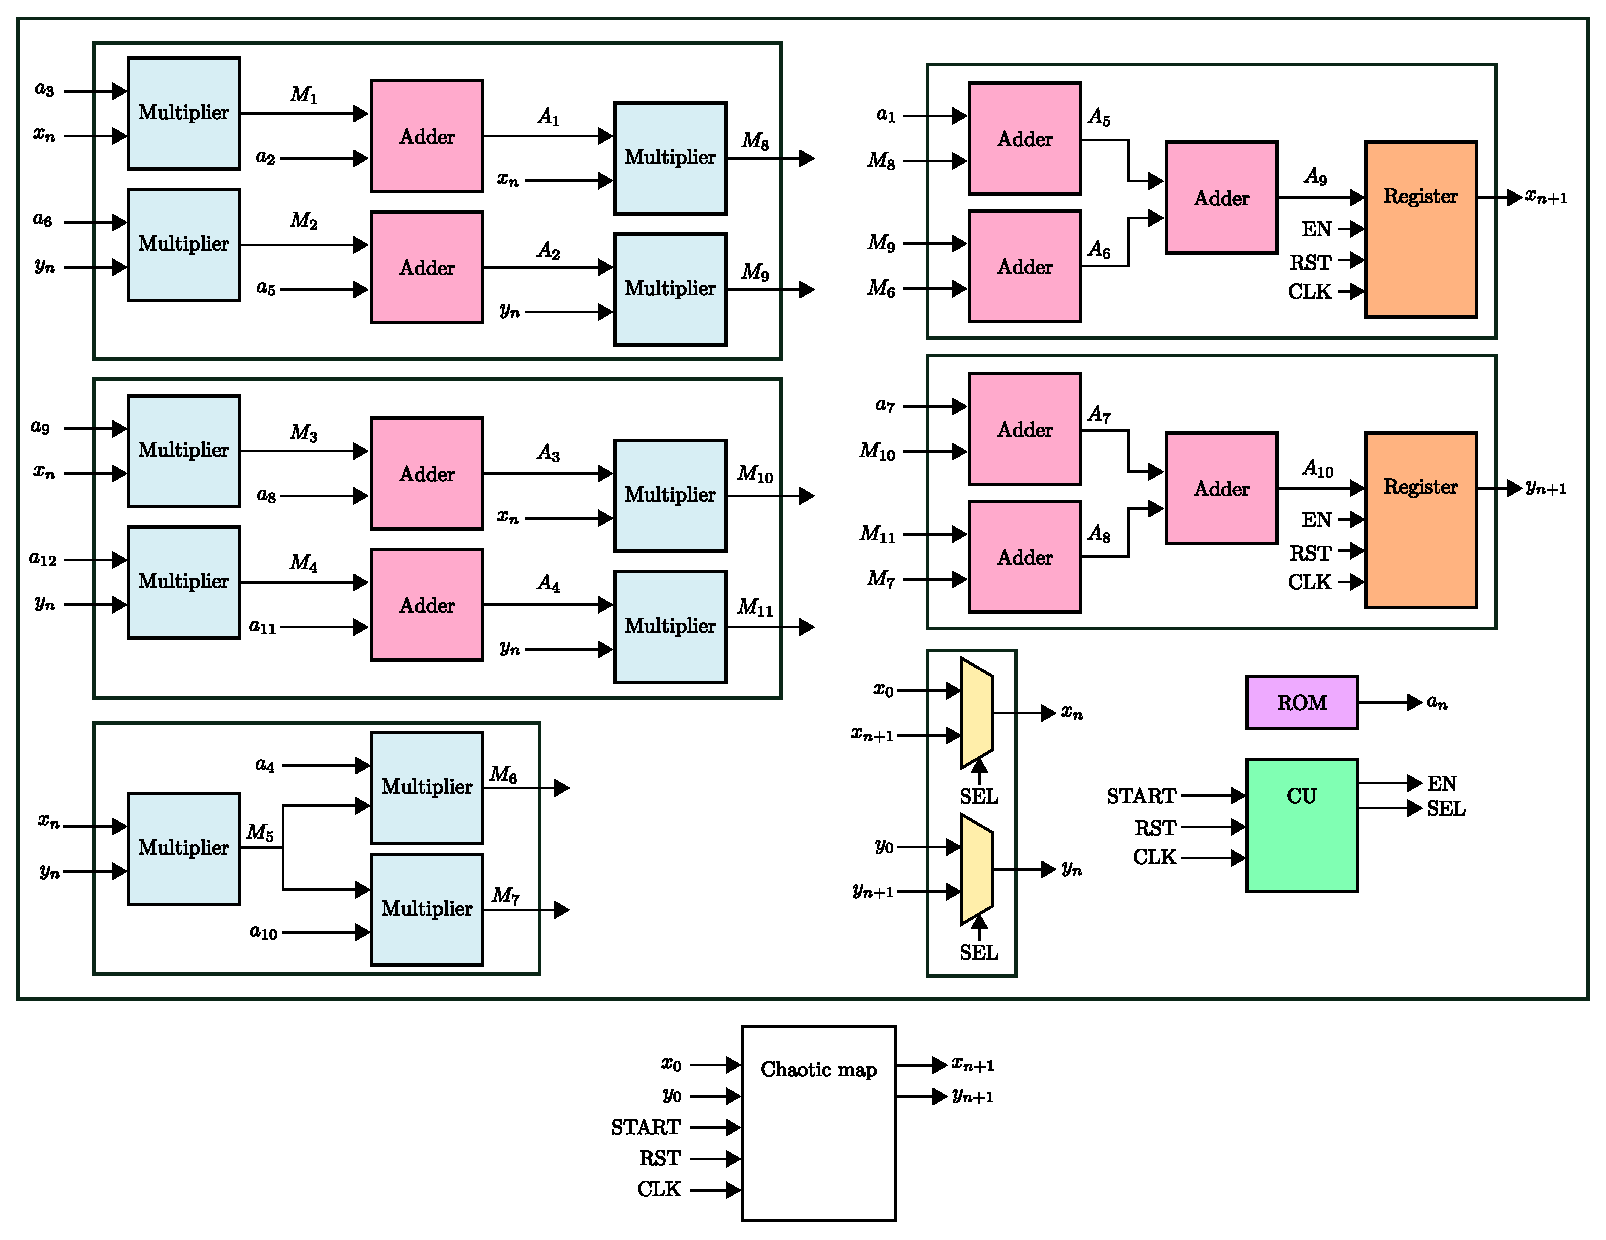
\includegraphics[width=0.9\linewidth]{B1_architecture}
		\label{fig:B1_architecture}
	\end{figure}
	
	
	\begin{figure}[hbtp]
		\caption{Máquina de estados de mapa caótico.}
		\centering
		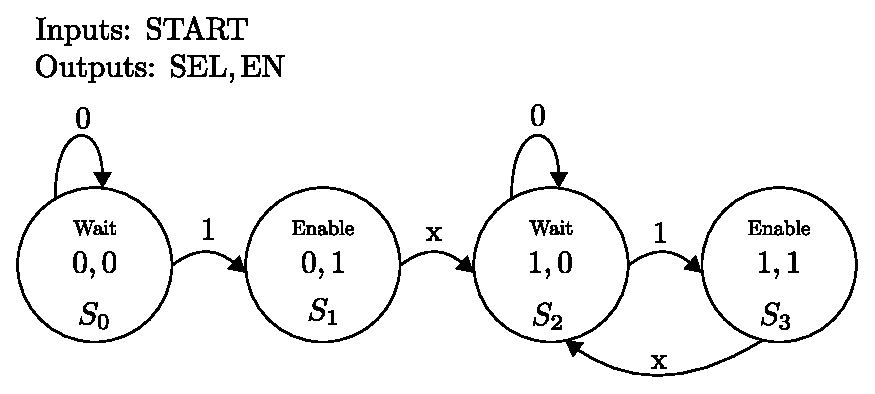
\includegraphics[width=0.6\linewidth]{B2_fsm_cm}
		\label{fig:B2_fsm_cm}
	\end{figure}
	
	
	Simulación del sistema en punto flotante en C
	
	\begin{figure}[hbtp]
		\caption{Mapa caótico.}
		\centering
		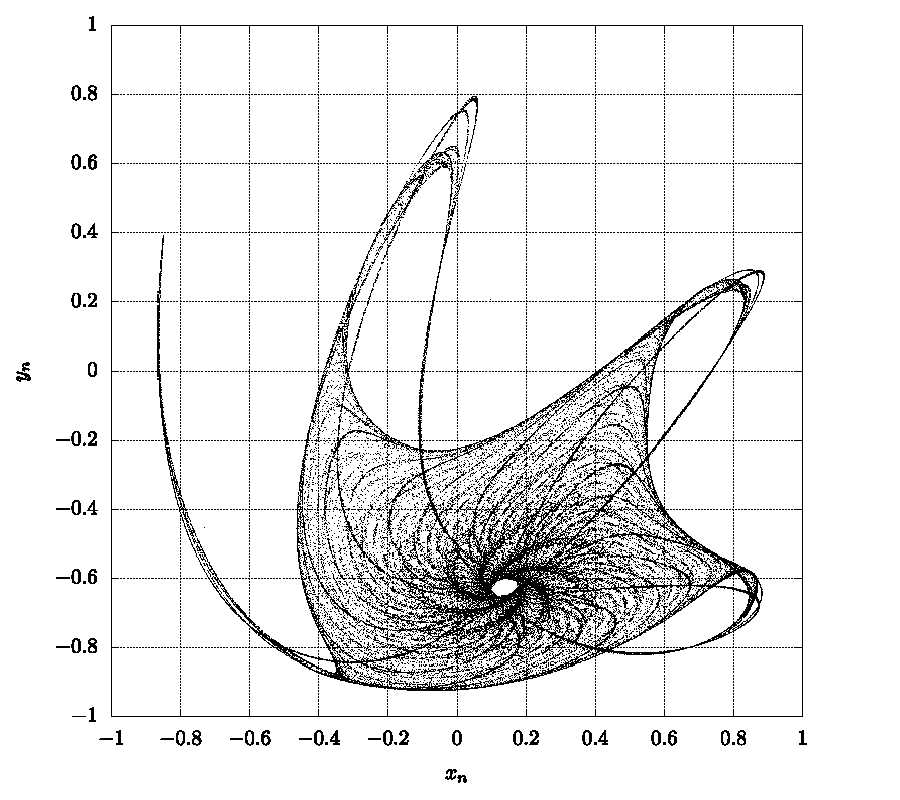
\includegraphics[width=0.8\linewidth]{B0_chaotic_map}
		\label{fig:B0_chaotic_map}
	\end{figure}
	
	
	
	\section{Comunicación RS232}
	
	\begin{figure}[hbtp]
		\caption{Máquina de estados para transmisión.}
		\centering
		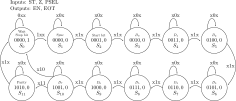
\includegraphics[width=0.8\linewidth]{C0_fsm_rs232}
		\label{fig:C0_fsm_rs232}
	\end{figure}	
	
	
	\begin{figure}[hbtp]
		\caption{Arquitectura de transmisión.}
		\centering
		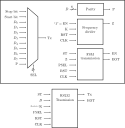
\includegraphics[width=0.6\linewidth]{C1_architecture_rs232}
		\label{fig:C1_architecture_rs232}
	\end{figure}
	
	\begin{figure}[hbtp]
		\caption{Arquitectura de TRNG.}
		\centering
		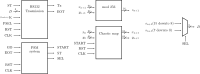
\includegraphics[width=0.9\linewidth]{D0_system}
		\label{fig:D0_system}
	\end{figure}
	
	\begin{figure}[hbtp]
		\caption{Máquina de estados de arquitectura de TRNG.}
		\centering
		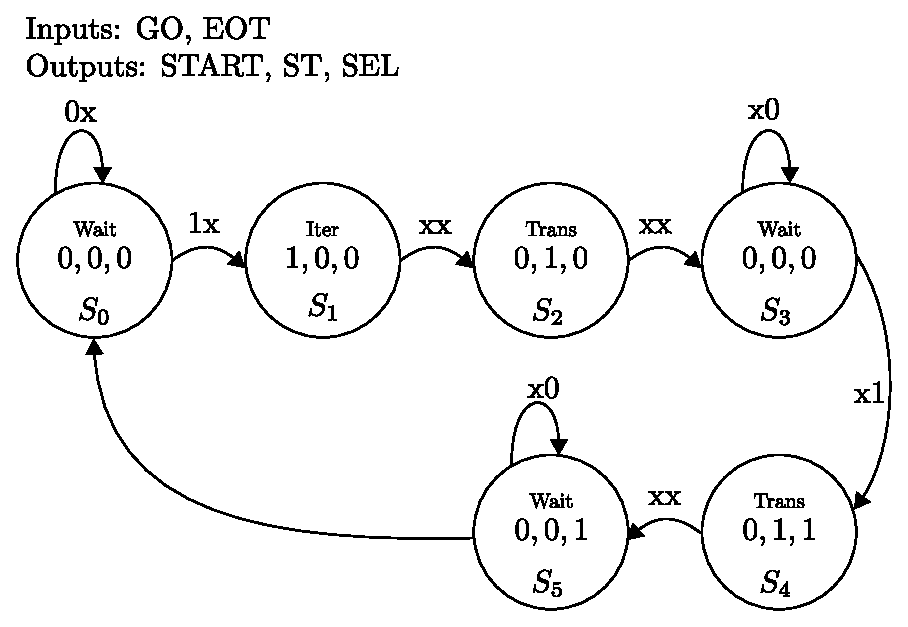
\includegraphics[width=0.7\linewidth]{D1_fsm_system}
		\label{fig:D1_fsm_system}
	\end{figure}
	

	
\begin{table}[htbp]
  \centering
  \caption{Resumen de los resultados de implementación de las TRNGs}
\resizebox{0.5\linewidth}{!}{ 
    \begin{tabular}{lll}
   & Test name                 & Prop. \\
   \hline
1  & Frequency                 & 0.99  \\
2  & Block frequency           & 0.99  \\
3  & Runs                      & 1.00     \\
4  & Longest run               & 1.0     \\
5  & Rank                      & 0.98  \\
6  & DFT                       & 0.99  \\
7  & Non-overlapping templates & 1.00     \\
8  & Overlapping templates     & 0.99  \\
9  & Universal                 & 0.99  \\
10 & Linear complexity         & 0.99  \\
11 & Serial                    & 0.99  \\
12 & Approximate Entropy       & 0.99  \\
13 & Cumulative Sums           & 0.99  \\
14 & Random excursions         & 0.99  \\
15 & Random excursions variant & 1.00    
    \end{tabular}
}
  \label{tab:asdasd}
\end{table}


\newpage
	Para poder realizar la implementación del núcleo ERO es necesario utilizar las primitivas y macros propias del fabricante de FPGA que para este trabajo es Xilinx. Las primitivas son componentes de Xilinx que son nativos de la arquitectura a la que se dirige y los macros son elementos que se encuentran en las bibliotecas UniMacro y Xilinx Parameterized Macros, las cuales se utilizan para instanciar elementos que son complejos de instanciar simplemente usando las primitivas, después las herramientas de síntesis expanden automáticamente estas macros a sus primitivas subyacentes. Los métodos de diseño disponibles son la instanciación, la inferencia, el catalogo IP y el soporte de macros, no obstante para este diseño solo se utilizan la instanciación, la cual permite instanciar un componente directamente en el diseño y es útil si se desea controlar el uso, la implementación y la ubicación exactos de los bloques individuales y el soporte de macros, el cual, utilizando las librerías antes mencionadas permiten abstraer la complejidad de utilizar unicamente primitivas simples.
	
	Toda la información referente a los macros y primitivas se encuentran en la documentación oficial en el archivo llamado ``Vivado Design Suite 7 Series FPGA Libraries Guide''. Para poder utilizar las primitivas y las macros es necesario agregar la librería UniMacro en la cabecera del archivo VHDL de la siguiente manera: 

\vspace{0.4cm}
\begin{lstlisting}[style = VHDL_TEXT]
LIBRARY UNISIM;
USE UNISIM.vcomponents.ALL;
\end{lstlisting}

	\section{Primitivas}
	
		\subsection{LUT1: 1-Bit Look-Up Table with General Output}
	
	\begin{figure}[hbtp]
		\caption{Esquemático de LUT1.}
		\centering
		\includegraphics[width=0.3\linewidth]{D3_lut1}
		\label{fig:D2_lut1}
	\end{figure}	
	
Este elemento proporciona una versión de look-up table de un búfer o inversor. Estos elementos son los bloques de construcción básicos. El parámetro INIT le da a la LUT su valor lógico. De forma predeterminada, este valor es cero, lo que lleva la salida a cero independientemente de los valores de entrada (actuando como tierra).Sin embargo, en la mayoría de los casos hay que determinar un nuevo valor INIT para especificar la función lógica de la primitiva LUT. Existen al menos dos métodos mediante los cuales se puede determinar el valor LUT. El método de la tabla lógica y el método de ecuación. En la Tabla \ref{tab:lut1} se muestran las entradas y salidas y la forma de configurar INIT y en el Código \ref{cod:lut1} se muestra su implementación en VHDL.


	\begin{table}[htbp]
		\centering
		\caption{Tabla lógica de LUT1.}
		\begin{tabular}{|cc|}
		\hline
		\multicolumn{1}{|c|}{\textbf{Inputs}} & \textbf{Outputs} \\ 
		\multicolumn{1}{|c|}{\textbf{I0}} & \textbf{O} \\ \hline 
		\multicolumn{1}{|c|}{0} & INIT[0] \\ \hline
		\multicolumn{1}{|c|}{1} & INIT[1] \\ \hline
		\multicolumn{2}{|c|}{INIT = Binary number assigned to the INIT attribute}          \\ \hline
		\end{tabular}
		\label{tab:lut1}
	\end{table}	
	

\vspace{0.4cm}
\begin{lstlisting}[style = VHDL_TEXT, caption = Primitiva LUT1., label = cod:lut1]
Library UNISIM;
use UNISIM.vcomponents.all;
-- LUT1: 1-input Look-Up Table with general output
-- 7 Series
-- Xilinx HDL Language Template, version 2021.2
LUT1_inst : LUT1
generic map (
    INIT => "00")
port map (
    O => O, -- LUT general output
    I0 => I0 -- LUT input
);
-- End of LUT1_inst instantiation
\end{lstlisting}






	\subsection{OBUFDS: Differential Signaling Output Buffer}
	
	\begin{figure}[hbtp]
		\caption{Esquemático de OBUFDS.}
		\centering
		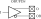
\includegraphics[width=0.3\linewidth]{D3_obufds}
		\label{fig:D3_obufds}
	\end{figure}	
	
	Este elemento de diseño es un búfer de salida única que admite señalización diferencial de bajo voltaje. OBUFDS aísla el circuito interno y proporciona corriente de accionamiento para las señales que salen del chip. Su salida se representa como dos puertos distintos (O y OB), uno considerado el ``maestro'' y el otro el ``esclavo''. El maestro y el esclavo son fases opuestas de la misma señal lógica.  En la Tabla \ref{tab:obufsd} se muestran las entradas y salidas y en el Código \ref{cod:obufsd} se muestra su implementación en VHDL.

	
	\begin{table}[htbp]
		\centering
		\caption{Tabla lógica de OBUFDS.}
		\begin{tabular}{|c|cc|}
		\hline
		\textbf{Inputs} & \multicolumn{2}{c|}{\textbf{Outputs}} \\ 
		\textbf{I}      & \multicolumn{1}{c}{\textbf{O}}  & \textbf{OB} \\ \hline
		0      & \multicolumn{1}{c|}{0}  & 1  \\ \hline
		1      & \multicolumn{1}{c|}{1}  & 0  \\ \hline
		\end{tabular}
		\label{tab:obufsd}
	\end{table}


\vspace{0.4cm}
\begin{lstlisting}[style = VHDL_TEXT, caption = Primitiva OBUFDS., label = cod:obufsd]
Library UNISIM;
use UNISIM.vcomponents.all;
-- OBUFDS: Differential Output Buffer
-- 7 Series
-- Xilinx HDL Language Template, version 2021.2
OBUFDS_inst : OBUFDS
generic map (
    IOSTANDARD => "DEFAULT", -- Specify the output I/O standard
    SLEW => "SLOW") -- Specify the output slew rate
port map (
    O => O, -- Diff_p output (connect directly to top-level port)
    OB => OB, -- Diff_n output (connect directly to top-level port)
    I => I -- Buffer input
);
-- End of OBUFDS_inst instantiation
\end{lstlisting}



Datos para programar la tarjeta

Default Board: Basys3
Default Part: xc7a35tcpg236-1
Product: Artix-7
Family: Artix-7
Package: cpg236
Speed Grade: -1







